\chapter{Basic Usage}
\label{chap:BasicUsage}

Let us get started using ParaView.  In order to follow along, you will need
your own installation of ParaView.  Specifically, this document is based
off of ParaView version \pvversion.  If you do not already have ParaView
\pvversion, you can download a copy from
\href{http://www.paraview.org}{www.paraview.org} (click on the download
link).  ParaView launches like most other applications.  On Windows, the
launcher is located in the start menu.  On Macintosh, open the application
bundle that you installed.  On Linux, execute \commandline{paraview} from a
command prompt (you may need to set your path).

The examples in this tutorial also rely on some data that is available at
\href{http://www.paraview.org/Wiki/ParaView_Tutorial}{http://www.paraview.org/Wiki/ParaView\_Tutorial}.
You may install this data into any directory that you like, but make sure
that you can find that directory easily.  Any time the tutorial asks you to
load a file it will be from the directory you installed this data in.


\section{User Interface}

\begin{inlinefig}
  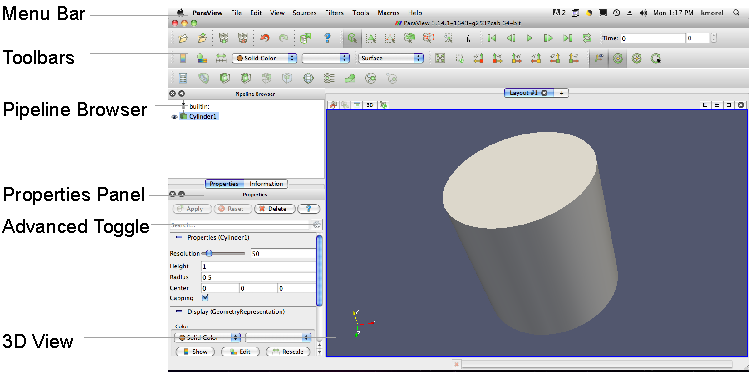
\includegraphics[scale=\bbscale]{images/UserInterface}
\end{inlinefig}

The ParaView GUI conforms to the platform on which it is running, but on
all platforms it behaves basically the same.  The layout shown here is the
default layout given when ParaView is first started.  The GUI comprises the
following components.

\begin{description}
\item[Menu Bar] \index{menu bar} As with just about any other program, the
  menu bar allows you to access the majority of features.
\item[Toolbars] \index{toolbars} The toolbars provide quick access to the
  most commonly used features within ParaView.
\item[Pipeline Browser] \index{pipeline browser} ParaView manages the
  reading and filtering of data with a pipeline.  The pipeline browser
  allows you to view the pipeline structure and select pipeline objects.
  Redesigned for ParaView 3, the pipeline browser provides a convenient
  list of pipeline objects with an indentation style that shows the
  pipeline structure.
\item[Object Inspector] \index{object inspector} The object inspector
  allows you to view and change the parameters of the current pipeline
  object.  There are three tabs in the object inspector.  The
  \keyterm{Properties} tab presents the configurable options for the object
  behavior.  The \keyterm{Display} tab presents options for how the object
  is represented in the view.  The \keyterm{Information} tab shows basic
  statistics on the data produced by the pipeline object.
\item[3D View] \index{3D View} The remainder of the GUI is used to present
  data so that you may view, interact with, and explore your data.  This
  area is initially populated with a 3D view that will provide a geometric
  representation of the data.
\end{description}

Note that the GUI layout is highly configurable, so that it is easy to
change the look of the window.  The toolbars can be moved around and even
hidden from view.  To toggle the use of a toolbar, use the \gui{View} \ra
\gui{Toolbars} submenu.  The pipeline browser and object inspector are both
\keyterm{dockable} windows.  This means that these components can be moved
around in the GUI, torn off as their own floating windows, or hidden
altogether.  These two windows are important to the operation of ParaView,
so if you hide them and then need them again, you can get them back with
the \gui{View} menu.


\section{Sources}

There are two ways to get data into ParaView: read data from a file or
generate data with a \keyterm{source} object.  All sources are located in
the \gui{Sources} menu.  Sources can be used to add annotation to a view,
but they are also very handy when exploring ParaView’s features.

\begin{exercise}{Creating a Source}
  \label{ex:CreatingASource}%
  Let us start with a simple one.  Go to the \gui{Sources} menu and select
  \gui{Cylinder}.  Once you select the \gui{Cylinder} item you will notice
  that an item named \gui{Cylinder1} is added to and selected in the
  pipeline browser.  You will also notice that the object inspector is
  filled with the properties for the cylinder source.  Click the
  \gui{Apply} button \apply to accept the default parameters.

  Once you click \gui{Apply}, the cylinder object will be displayed in the
  3D view window on the right.  You can manipulate this 3D view by dragging
  the mouse over the 3D view.  Experiment with dragging different mouse
  buttons---left, middle, and right---to perform different rotate, pan, and
  zoom operations.  Also try using the buttons in conjunction with the
  shift and ctrl modifier keys.

  You will quickly notice that ParaView creates not a real cylinder but
  rather an approximation of a cylinder using polygonal \keyterm{facets}.
  The default parameters for the cylinder source provide a very coarse
  approximation of only six facets. (In fact, this object looks more like a
  prism than a cylinder.) If we want a better representation of a cylinder,
  we can create one by increasing the \gui{Resolution} parameter.

  \begin{inlinefig}
    \includegraphics[width=.83\scw]{images/ResolutionParameter}
  \end{inlinefig}

  Using either the slider or text edit, increase the resolution to 50 or
  more.  Notice that the \gui{Apply} button \apply has turned green (or
  blue on Mac) again.  This is because changes you make to the object
  inspector are not immediately enacted.  The highlighted button is a
  reminder that the parameters of one or more pipeline objects are ``out of
  sync'' with the data that you are viewing.  Hitting the \gui{Apply} button
  will accept these changes whereas hitting the \gui{Reset} button \reset
  will revert the options back to the last time they were applied.  Hit the
  \gui{Apply} button now.  The resolution is changed so that it is
  virtually indistinguishable from a true cylinder.
\end{exercise}

Now is a good time to note the undo~\icon{pqUndo32} and
redo~\icon{pqRedo32} buttons in the toolbar.  Visualizing your data is
often an exploratory process, and it is often helpful to revert back to a
previous state.  You can even undo back to the point before your data was
created and redo again.

\begin{exercise}{Undo and Redo}
  \label{ex:UndoAndRedo}%
  Experiment with the undo~\icon{pqUndo32} and redo~\icon{pqRedo32}
  buttons.  If you have not done so, create and modify a pipeline object
  like what is done in Exercise~\ref{ex:CreatingASource}.  Watch how
  parameter changes can be reverted and restored.  Also notice how whole
  pipeline objects can be destroyed and recreated.

  There are also undo camera~\icon{pqUndoCamera24} and redo
  camera~\icon{pqRedoCamera24} buttons.  These allow you to go back and
  forth between camera angles that you have made so that you no longer have
  to worry about errant mouse movements ruining that perfect view.  Move
  the camera around and then use these buttons to revert and restore the
  camera angle.
\end{exercise}

There are also many options for selecting how objects are rendered.  You
will notice over the 3D view a \icon{pqOptions16} button for changing the
rendering options.  Clicking this brings up a dialog box that allows you to
change things like the background color, the lighting, and annotation.

\begin{inlinefig}
  \includegraphics[width=\scw]{images/RenderViewOptions}
\end{inlinefig}

Another location for rendering options is the \gui{Display} tab in the
object inspector.  This tab provides the rendering options that apply
specifically for the selected object.  It includes the visibility,
coloring, and representation.  Be aware that some of the view options and
object display options are repeated elsewhere in the ParaView GUI for
convenience.

\begin{inlinefig}
  \includegraphics[width=0.53\scw]{images/DisplayTab}
\end{inlinefig}

\begin{exercise}{Modifying Rendering Parameters}
  \label{ex:ModifyingRenderingParameters}%
  Click the \icon{pqOptions16} button above the 3D view to bring up the
  \gui{Render View Options} dialog box.  Explore the different panels of
  options.  Try modifying how the view looks in the following ways.
  (Remember that you will have to hit \gui{Apply} or \gui{OK} before the
  changes take effect.)

  \begin{itemize}
  \item Change the background color.  (Notice that you can reset it to the
    default.)
  \item Turn the Orientation Axis (the axis in the lower left corner of the
    view) off and on.
  \item Move the Orientation Axis in the view.  (Hint: Make the axis
    interactive and then click and drag in the 3D view.)
  \end{itemize}

  Now change the drawing parameters of the cylinder.  (If you do not have a
  cylinder or another pipeline object, create one as described in
  Exercise~\ref{ex:CreatingASource}.)  Make sure the cylinder is selected
  in the pipeline browser.  In the object inspector, select the
  \gui{Display} tab.

  \begin{itemize}
  \item Set the (solid) color of the cylinder.  (Note: You can also set the
    color with the \icon{pqEditColor24} toolbar button.)
  \item Make the cylinder shiny.  (Hint: Make the \gui{Specular Intensity}
    1.0.)
  \item Make the cylinder transparent.  (Hint: Lower the \gui{Opacity}.)
  \item Show 3D axes with tic marks giving spatial position (\gui{Show cube
    axes}).
  \end{itemize}

  We are done with the cylinder source now.  We can delete the pipeline
  object by selecting the \gui{Properties} tab and hitting delete \delete
  in the object inspector.
\end{exercise}


\section{Loading Data}

Now that we have had some practice using the ParaView GUI, let us load in
some real data.  As you would expect, the \gui{Open} command is the first
one off of the \gui{File} menu, and there is also toolbar
button~\icon{pqOpen32} for opening a file.  ParaView supports many file
types, and the list grows as more types get added.  The following is a list
of currently available readers.

% Multicols does not work correctly when in twocolumn mode and it breaks
% across page boundaries.  That's too bad since it saves space and looks
% nice.
\ifthenelse{\boolean{savetrees}}{
}{
  \begin{multicols}{2}
}
  \begin{itemize}
  \item ParaView Data (.pvd)
  \item VTK (.vtp, .vtu, .vti, .vts, .vtr)
  \item VTK Multi Block (.vtm, .vtmb, .vtmg, .vthd, .vthb)
  \item Partitioned VTK (.pvtu, .pvti, .pvts, .pvtr)
  \item VTK Legacy (.vtk)
  \item Exodus
  \item XDMF and hdf5 (.xmf, .xdmf)
  \item LS-DYNA
  \item SpyPlot CTH
  \item EnSight (.case, .sos)
  \item netCDF (.ncdf, .nc)
  \item BYU (.g)
  \item Protein Data Bank (.pdb)
  \item XMol Molecule
  \item PLOT3D
  \item Digital Elevation Map (.dem)
  \item VRML (.wrl)
  \item PLY Polygonal File Format
  \item Stereo Lithography (.stl)
  \item Gaussian Cube File (.cube)
  \item POP Ocean Files
  \item AVS UCD (.inp)
  \item Meta Image (.mhd, .mha)
  \item Facet Polygonal Data
  \item Phasta Files (.pht)
  \item SESAME Tables
  \item MFIX (.RES)
  \item Fluent Case Files (.cas)
  \item OpenFOAM Files (.foam)
  \item Cosmology Files (.cosmo)
  \item PNG Image Files
  \item TIFF Image Files
  \item Raw Image Files
  \item Comma Separated Values (.csv)
  \item Wavefront Polygonal Data (.obj)
  \item Spy Plot (.case)
  \item Enzo boundary and hierarchy
  \item Flash multiblock files
  \item Raw NRRD image files (.nrrd)
  \item LANL cosmology data (.cosmo)
  \item VPIC (.vpc)
  \item SLAC netCDF mesh and mode data
  \item SLAC netCDF particle data
  \item LANL windbade (.wind)
  \item Tecplot ASCII (.tec, .tp)
  \end{itemize}
\ifthenelse{\boolean{savetrees}}{
}{
  \end{multicols}
}

ParaView's modular design allows for easy integration of new VTK readers
into ParaView.  Thus, check back often for new file formats.  If you are
looking for a file reader that does not seem to be included with ParaView,
check in with the ParaView mailing list
(\href{mailto:paraview@paraview.org}{paraview@paraview.org}).  There are
many file readers included with VTK but not exposed within ParaView that
could easily be added.  There are also many readers created that can plug
into the VTK framework but have not been committed back to VTK; someone may
have a reader readily available that you can use.

\begin{exercise}{Opening a File}
  \label{ex:OpeningAFile}%
  Let us open our first file now.  Click the \gui{Open} toolbar (or menu
  item)~\icon{pqOpen32} and open the file \gui{disk\_out\_ref.ex2}.  Note
  that opening a file is a two step process, so that you do not see any
  data yet.  Instead, you see that the object inspector is populated with
  several options about how we want to read the data.

  \begin{inlinefig}
    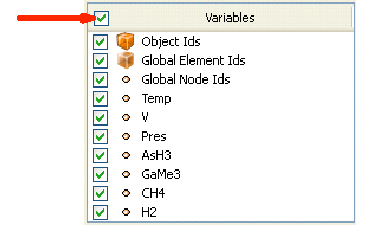
\includegraphics[scale=\bbscale]{images/Variables_disk_out_ref}
  \end{inlinefig}

  Click the checkbox in the header of the variable list to turn on the
  loading of all the variables.  This is a small data set, so we do not
  have to worry about loading too much into memory.  Once all of the
  variables are selected, click \apply to load all of the data.  When the
  data is loaded you will see that the geometry looks like a cylinder with
  a hollowed out portion in one end.  This data is the output of a
  simulation for the flow of air around a heated and spinning disk.  The
  mesh you are seeing is the air around the disk (with the cylinder shape
  being the boundary of the simulation.  The hollow area in the middle is
  where the heated disk would be were it meshed for the simulation.
\end{exercise}

Before we continue on to filtering the data, let us take a quick look at
some of the ways to represent the data.  The most common parameters for
representing data are located in a pair of toolbars.

\begin{inlinefig}
  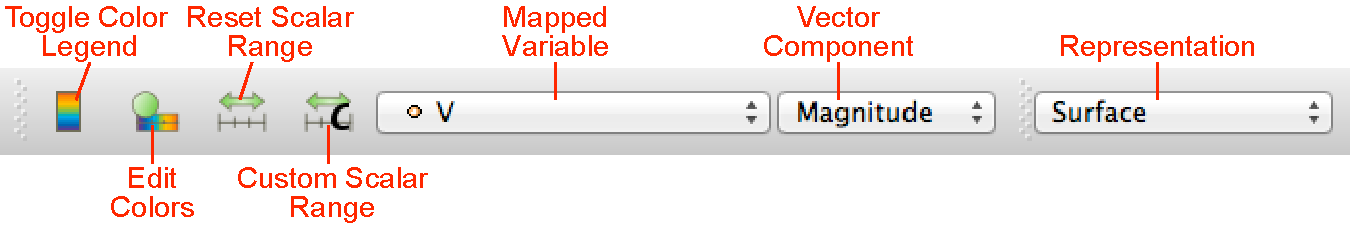
\includegraphics[width=\linewidth]{images/DataRepresentationToolbars}
\end{inlinefig}

\begin{exercise}{Representation and Field Coloring}
  \label{ex:RepresentationAndFieldColoring}%
  Play with the data representation a bit.  Make sure
  \gui{disk\_out\_ref.ex2} is selected in the pipeline browser.  (If you do
  not have the data loaded, repeat Exercise~\ref{ex:OpeningAFile}.)  Use
  the variable chooser to color the surface by the \gui{Pres} variable.
  Then turn the color legend on to see the actual pressure values.  To see
  the structure of the mesh, change the representation to \gui{Surface With
    Edges}.  You can view both the cell structure and the interior of the
  mesh with the \gui{Wireframe} representation.

  \begin{inlinefig}
    \includegraphics[width=.42\linewidth]{images/DataRepresentation1}
    \includegraphics[width=.42\linewidth]{images/DataRepresentation2} \\
    \includegraphics[width=.42\linewidth]{images/DataRepresentation3}
    \includegraphics[width=.42\linewidth]{images/DataRepresentation4}
  \end{inlinefig}
\end{exercise}


\section{Filters}

We have now successfully read in some data and gleaned some information
about it.  We can see the basic structure of the mesh and map some data
onto the surface of the mesh.  However, as we will soon see, there are many
interesting features about this data that we cannot determine by simply
looking at the surface of this data.  There are many variables associated
with the mesh of different types (scalars and vectors).  And remember that
the mesh is a solid model.  Most of the interesting information is on the
inside.

We can discover much more about our data by applying \keyterm{filters}.
Filters are functional units that process the data to generate, extract, or
derive features from the data.  Filters are attached to readers, sources,
or other filters to modify its data in some way.  These filter connections
form a \keyterm{visualization pipeline}.  There are a great many filters
available in ParaView.  Here are the most common, which are all available
by clicking on the respective icon in the filters toolbar.

\begin{description}
\item[\calculator Calculator] \index{calculator} Evaluates a user-defined
  expression on a per-point or per-cell basis.
\item[\contour Contour] \index{contour} Extracts the points, curves, or
  surfaces where a scalar field is equal to a user-defined value.  This
  surface is often also called an \keyterm{isosurface}.
\item[\clip Clip] \index{clip} Intersects the geometry with a half space.
  The effect is to remove all the geometry on one side of a user-defined
  plane.
\item[\slice Slice] \index{slice} \index{cut|see{slice}} Intersects the
  geometry with a plane.  The effect is similar to clipping except that all
  that remains is the geometry where the plane is located.
\item[\threshold Threshold] \index{threshold} Extracts cells that lie
  within a specified range of a scalar field.
\item[\extractSubset Extract Subset] \index{extract subset} Extracts a
  subset of a grid by defining either a volume of interest or a sampling
  rate.
\item[\glyph Glyph] Places a \keyterm{glyph}, a simple shape, on each point
  in a mesh.  The glyphs may be oriented by a vector and scaled by a vector
  or scalar.
\item[\streamTracer Stream Tracer] \index{stream tracer} Seeds a vector
  field with points and then traces those seed points through the (steady
  state) vector field.
\item[\warp Warp (vector)] \index{warp!vector} Displaces each point in a
  mesh by a given vector field.
\item[\group Group Datasets] \index{group datasets} Combines the output of
  several pipeline objects into a single multi block data set.
\item[\extractGroup Extract Level] \index{extract level} Extract one or
  more items from a multi block data set.
\end{description}

\parpic[r]{\includegraphics[width=0.37\scw]{images/FiltersMenu}}

These eleven filters are a small sampling of what is available in ParaView.
In the \gui{Filters} menu are a great many more filters that you can use to
process your data.  ParaView currently exposes more than one hundred filters, so to
make them easier to find the \gui{Filters} menu is organized into submenus.
These submenus are organized as follows.

\begin{description}
\item[Recent] The list of most recently used filters sorted with the most
  recently used filters on top.
\item[Common] The most common filters.  This is the same list of filters
  available in the filters toolbar and listed previously.
\item[Cosmology] This contains filters developed at LANL for cosmology research. 
\item[Data Analysis] The filters designed to retrieve quantitative values
  from the data.  These filters compute data on the mesh, extract elements
  from the mesh, or plot data.
\item[Statistics] This contains filters that provide descriptive
  statistics of data, primarily in tabular form.
\item[Temporal] Filters that analyze or modify data that changes over time.
  All filters can work on data that changes over time because they are
  executed on each time snapshot.  However, filters in this category will
  introspect the available time extents and examine how data changes over
  time.
\item[Alphabetical] An alphabetical listing of all the filters available.
  If you are not sure where to find a particular filter, this list is
  guaranteed to have it.  There are also many filters that are not listed
  anywhere but in this list.
\end{description}

\parpic[r]{\includegraphics[width=.5\linewidth]{images/QuickLaunch}}

Searching through these lists of filters, particularly the full
alphabetical list, can be cumbersome.  To speed up the selection of
filters, you should use the \keyterm{quick launch} dialog.  When the ctrl
and space keys together on Windows or Linux or the alt and space keys
together on Macintosh, ParaView brings up a small, lightweight dialog box
like the one shown here.  Type in words or word fragments that are
contained in the filter name, and the box will list only those sources and
filters that match the terms.  Hit enter to add the object to the pipeline
browser.

You have probably noticed that some of the filters are grayed out.  Many
filters only work on a specific types of data and therefore cannot always
be used.  ParaView disables these filters from the menu and toolbars to
indicate (and enforce) that you cannot use these filters.

Throughout this tutorial we will explore many filters.  However, we cannot
explore all the filters in this forum.  Consult the Filters Menu
chapter of ParaView's on-line or in-built help for more information on each filter.

\begin{exercise}{Apply a Filter}
  \label{ex:ApplyAFilter}%
  Let us apply our first filter.  If you do not have the disk\_out\_ref.ex2
  data loaded, do so know (Exercise~\ref{ex:OpeningAFile}).  Make sure that
  \gui{disk\_out\_ref.ex2} is selected in the pipeline browser and then
  select the contour filter~\contour from the filter toolbar or
  \gui{Filters} menu.  Notice that a new item is added to the pipeline
  filter underneath the reader and the object inspector updates to the
  parameters of the new filter.  As with reading a file, applying a filter
  is a two step process.  After creating the filter you get a chance to
  modify the parameters (which you will almost always do) before applying
  the filter.

  \begin{inlinefig}
    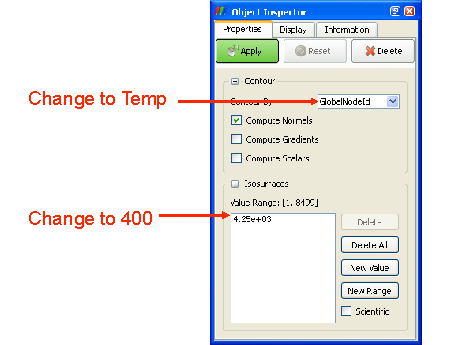
\includegraphics[scale=\bbscale]{images/ContourOptions}
  \end{inlinefig}

  We will use the contour filter to create an isosurface where the
  temperature is equal to 400 K.  First, change the \gui{Contour By}
  parameter to the \gui{Temp} variable.  Then, change the isosurface value
  to \gui{400}.  Finally, hit \apply.  You will see the isosurface appear
  inside of the volume.  If \gui{disk\_out\_ref.ex2} was still colored by
  pressure from Exercise~\ref{ex:RepresentationAndFieldColoring}, then the
  surface is colored by pressure to match.

  \begin{inlinefig}
    \includegraphics[width=\scw]{images/ContourResults}
  \end{inlinefig}
\end{exercise}

In the preceding exercise, we applied a filter that processed the data and
gave us the results we needed.  For most common operations, a single filter
operation is sufficient to get the information we need.  However, filters
are of the same class as readers.  That is, the general operations we apply
to readers can also be applied to filters.  Thus, you can apply one filter
to the data that is generated by another filter.  These readers and filters
connected together form what we call a \keyterm{visualization pipeline}.
The ability to form visualization pipelines provides a powerful mechanism
for customizing the visualization to your needs.

Let us play with some more filters.  Rather than show the mesh surface in
wireframe, which often interferes with the view of what is inside it, we
will replace it with a cutaway of the surface.  We need two filters to
perform this task.  The first filter will extract the surface, and the
second filter will cut some away.

\begin{exercise}{Creating a Visualization Pipeline}
  \label{ex:CreatingAVisualizationPipeline}%
  The images and some of the discussion in this exercise assume you are
  starting with the state right after finishing
  Exercise~\ref{ex:ApplyAFilter}.  If you have had to restart ParaView
  since or your state does not match up well enough, it is sufficient to
  simply have disk\_out\_ref.ex2 loaded.

  Start by adding a filter that will extract the surfaces.  We do that with
  the following steps.

  \begin{enumerate}
  \item Select \gui{disk\_out\_ref.ex2} in the pipeline browser.
  \item From the menu bar, select \gui{Filters} \ra \gui{Alphabetical} \ra
    \gui{Extract Surface}. \index{extract surface} Or bring up the quick
    launch (ctrl+space Win/Linux, alt+space Mac), type extract surface, and
    select that filter.
  \item Hit the \apply button.
    \savecounter
  \end{enumerate}

  \begin{inlinefig}
    \includegraphics[width=\scw]{images/CutSurface1}
  \end{inlinefig}

  When you apply the \gui{Extract Surface} filter, you will once again see
  the surface of the mesh.  Although it looks like the original mesh, it is
  different in that this data is hollow whereas the original data was solid
  throughout.

  If you were showing the results of the contour filter, you cannot see the
  contour anymore, but do not worry.  It is still in there hidden by the
  surface.  If you are showing the contour but you did not see any effect
  after applying the filter, you may have forgotten step one and applied
  the filter to the wrong object.  If the \gui{ExtractSurface1} object is
  not connected directly to the \gui{disk\_out\_ref.ex2}, then this is what
  went wrong.  If so, you can delete the filter and try again.

  Now we will cut away the external surface to expose the internal
  structure and isosurface underneath (if you have one).

  \begin{enumerate}
    \restorecounter
  \item Verify that \gui{ExtractSurface1} is selected in the pipeline
    browser.
  \item Create a clip filter \clip from the toolbar or \gui{Filters} menu.
  \item Uncheck the \gui{Show Plane} checkbox
    \includeinlinegraphics{images/ShowPlaneCheckbox} in the object inspector.
  \item Click the \apply button.
  \end{enumerate}

  \begin{inlinefig}
    \includegraphics[width=\scw]{images/CutSurface2}
  \end{inlinefig}

  If you have a contour, you should now see the isosurface contour within a
  cutaway of the mesh surface.  You will probably have to rotate the mesh
  to see the contour clearly.
\end{exercise}

\begin{inlinefig}
  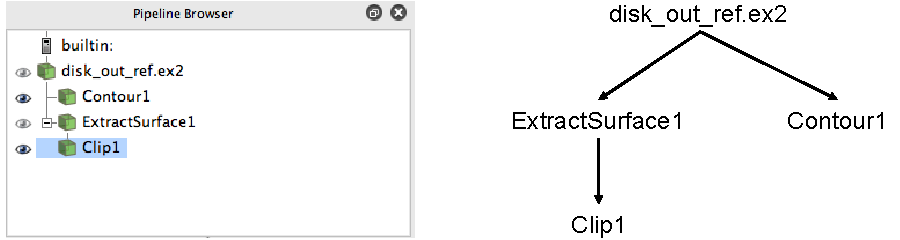
\includegraphics[width=\linewidth]{images/PipelineBrowserStructure}
\end{inlinefig}

Now that we have added several filters to our pipeline, let us take a look
at the layout of these filters in the pipeline browser.  The pipeline
browser provides a convenient list of pipeline objects that we have created
make it easy to select pipeline objects and change their
\keyterm{visibility} by clicking on the eyeball icons~\eyeball next to
them.  But also notice the indentation of the entries in the list and the
connecting lines toward the right.  These features reveal the
\keyterm{connectivity} of the pipeline.  It shows the same information as
the traditional graph layout on the right, but in a much more compact
space.  The trouble with the traditional layout of pipeline objects is that
it takes a lot of space, and even moderately sized pipelines require a
significant portion of the GUI to see fully.  The pipeline browser,
however, is complete and compact.


\section{Multiview}
\label{sec:Multiview}

Occasionally in the pursuit of science we can narrow our focus down to one
variable.  However, most interesting physical phenomena rely on not one but
many variables interacting in certain ways.  It can be very challenging to
present many variables in the same view.  To help you explore complicated
visualization data, ParaView contains the ability to present multiple views
of data and correlate them together.

So far in our visualization we are looking at two variables: We are
coloring with pressure and have extracted an isosurface with temperature.
Although we are starting to get the feel for the layout of these variables,
it is still difficult to make correlations between them.  To make this
correlation easier, we can use multiple views.  Each view can show an
independent aspect of the data and together they may yield a more complete
understanding.

On top of each view is a small toolbar, and the buttons controlling the
creating and deletion of views are located on the right side of this tool
bar.  There are four buttons in all.  You can create a new view by
splitting an existing view horizontally or vertically with the \splitViewH
and \splitViewV buttons, respectively.  The \deleteView button deletes a
view, whose space is consumed by an adjacent view.  The \maximizeView
temporarily fills view space with the selected view until \restoreView is
pressed.

\begin{exercise}{Using Multiple Views}
  \label{ex:UsingMultipleViews}%
  We are going to start a fresh visualization, so if you have been
  following along with the exercises so far, now is a good time to reset
  ParaView.  The easiest way to do this is to press the~\disconnect button.
  We will discuss what this does later in more detail in
  Chapter~\ref{chap:VisualizingLargeModels}, but for now just know that it
  is roughly the equivalent of restarting ParaView.

  First, we will look at one variable.  We need to see the variable through
  the middle of the mesh, so we are going to clip the mesh in half.

  \begin{enumerate}
  \item Open the file disk\_out\_ref.ex2, load all variables, \apply (see
    Exercise~\ref{ex:OpeningAFile}).
  \item Add the Clip filter~\clip to \gui{disk\_out\_ref.ex2}.
  \item Uncheck the Show Plane checkbox
    \includeinlinegraphics{images/ShowPlaneCheckbox} in the object inspector.
  \item Click the \apply button.
  \item Color the surface by pressure by changing the variable chooser (in
    the toolbar) from \gui{Solid Color} to \gui{Pres}.
    \savecounter
  \end{enumerate}

  Now we can see the pressure in a plane through the middle of the mesh.
  We want to compare that to the temperature on the same plane.  To do
  that, we create a new view to build another visualization.

  \begin{enumerate}
    \restorecounter
  \item Press the \splitViewH button.
  \end{enumerate}

  \begin{inlinefig}
    \includegraphics[width=\scw]{images/SplitView1}
  \end{inlinefig}

  The current view is split in half and the right side is blank, ready to
  be filled with a new visualization.  Notice that the view in the right
  has a blue border around it.  This means that it is the \keyterm{active
    view}.  Widgets that give information about and controls for a single
  view, including the pipeline browser and object inspector, follow the
  active view.  In this new view we will visualize the temperature of the
  mesh.

  \begin{enumerate}
  \item Make sure the blue border is still around the new, blank view (to
    the right).  You can make any view the active view by simply clicking
    on it.
  \item Turn on the visibility of the clipped data by clicking the
    eyeball~\eyeballg next to \gui{Clip1} in the pipeline browser.
  \item Color the surface by temperature by selecting \gui{Clip1} in the
    pipeline browser and changing the variable chooser (in the toolbar)
    from \gui{Solid Color} to \gui{Temp} (you may want to turn on the color
    bar at this point as well).
    \savecounter
  \end{enumerate}

  \begin{inlinefig}
    \includegraphics[width=\scw]{images/SplitView2}
  \end{inlinefig}

  We now have two views: one showing information about pressure and the
  other information about temperature.  We would like to compare these, but
  it is difficult to do because the orientations are different.  How are we
  to know how a location in one correlates to a location in the other?  We
  can solve this problem by adding a \keyterm{camera link} so that the two
  views will always be drawn from the same viewpoint.  Linking cameras is
  easy.

  \begin{enumerate}
    \restorecounter
  \item Right click on one of the views and select \gui{Link Camera...}
    from the pop up menu. (If you are on a Mac with no right mouse button,
    you can perform the same operation with the menu option \gui{Tools} \ra
    \gui{Add Camera Link...}.)
  \item Click in a second view.
  \item Try moving the camera in each view.
  \end{enumerate}

  \emph{Voil\`{a}}!  The two cameras are linked; each will follow the other.
  With the cameras linked, we can make some comparisons between the two
  views.  Click the~\xPlus button to get a straight-on view of the cross
  section.

  \begin{inlinefig}
    \includegraphics[width=\scw]{images/CameraLink}
  \end{inlinefig}

  Notice that the temperature is highest at the interface with the heated
  disk.  That alone is not surprising.  We expect the air temperature to be
  greatest near the heat source and drop off away from it.  But notice that
  at the same position the pressure is not maximal.  The air pressure is
  maximal at a position above the disk.  Based on this information we can
  draw some interesting hypotheses about the physical phenomenon.  We can
  expect that there are two forces contributing to air pressure.  The first
  force is that of gravity causing the upper air to press down on the lower
  air.  The second force is that of the heated air becoming less dense and
  therefore rising.  We can see based on the maximal pressure where these
  two forces are equal.  Such an observation cannot be drawn without
  looking at both the temperature and pressure in this way.
\end{exercise}

Multiview in ParaView is of course not limited to simply two windows.  Note
that each of the views has its own set of multiview buttons.  You can
create more views by using the split view buttons \splitViewH \splitViewV
to arbitrarily divide up the working space.  And you can delete views
\deleteView at any time.

The location of each view is also not fixed.  You are also able to swap two
views by clicking on one of the view toolbars (somewhere outside of where
the buttons are), holding down the mouse button, and dragging onto one of
the other views.  This will immediately swap the two views.

\begin{inlinefig}
  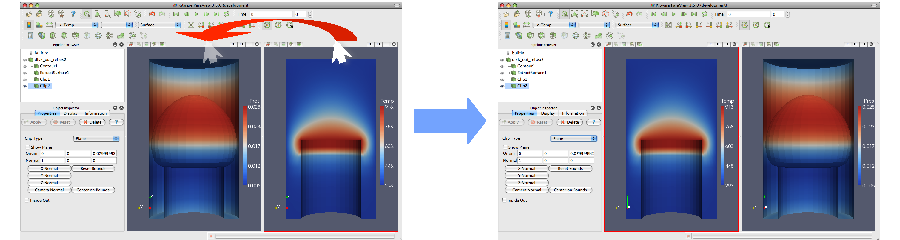
\includegraphics[width=\linewidth]{images/SwapViews}
\end{inlinefig}

You can also change the size of the views by clicking on the space in
between views, holding down the mouse button, and dragging in the direction
of either one of the views.  The divider will follow the mouse and adjust
the size of the views as it moves.

\begin{inlinefig}
  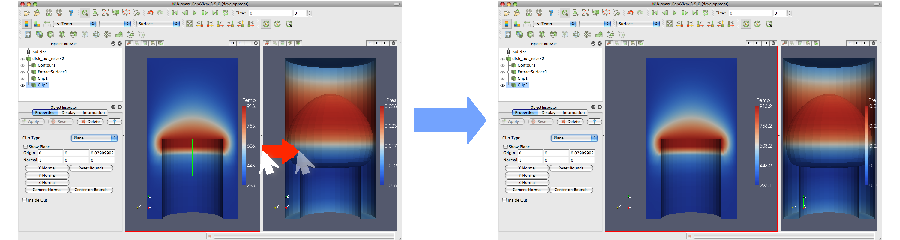
\includegraphics[width=\linewidth]{images/ResizeViews}
\end{inlinefig}


\section{Vector Visualization}

Let us see what else we can learn about this simulation.  The simulation
has also outputted a velocity field describing the movement of the air over
the heated rotating disk.  We will use ParaView to determine the currents
in the air.

A common and effective way to characterize a vector field is with
\keyterm{streamlines}.  A streamline is a curve through space that at every
point is tangent to the vector field.  It represents the path a weightless
particle will take through the vector field (assuming steady-state flow).
Streamlines are generated by providing a set of
\index{stream tracer!seed points} \keyterm{seed points}.

\begin{exercise}{Streamlines}
  \label{ex:Streamlines}%
  We are going to start a fresh visualization, so if you have been
  following along with the exercises so far, now is a good time to reset
  ParaView.  The easiest way to do this is to press the~\disconnect button.

  \begin{enumerate}
  \item Open the file disk\_out\_ref.ex2, load all variables, \apply (see
    Exercise~\ref{ex:OpeningAFile}).
  \item Add the stream tracer filter \streamTracer to
    \gui{disk\_out\_ref.ex2}.
  \item Click the \apply button to accept the default parameters.
  \end{enumerate}

  \begin{inlinefig}
    \includegraphics[width=\scw]{images/StreamTracer0}
  \end{inlinefig}

  The surface of the mesh is replaced with some swirling lines.  These
  lines represent the flow through the volume.  Notice that there is a
  spinning motion around the center line of the cylinder.  There is also a
  vertical motion in the center and near the edges.

  The new geometry is off-center from the previous geometry.  We can
  quickly center the view on the new geometry with the \keyterm{reset
    camera}~\resetCamera command.  This command centers and fits the
  visible geometry within the current view and also resets the center of
  rotation to the middle of the visible geometry.
\end{exercise}

One issue with the streamlines as they stand now is that the lines are
difficult to distinguish because there are many close together and they
have no shading.  Lines are a 1D structure and shading requires a 2D
surface.  Another issue with the streamlines is that we cannot be sure in which
direction the flow is.

In the next exercise, we will modify the streamlines we created in
Exercise~\ref{ex:Streamlines} to correct these problems.  We can create a
2D surface around our stream traces with the tube filter.  This surface
adds shading and depth cues to the lines.  We can also add glyphs to the
lines that point in the direction of the flow.

\begin{exercise}{Making Streamlines Fancy}
  \label{ex:MakingStreamlinesFancy}%
  \begin{enumerate}
  \item Use the quick launch (ctrl+space Win/Linux, alt+space Mac) to apply
    the \gui{Tube}\index{tube} filter.
  \item Hit the \apply button.
    \savecounter
  \end{enumerate}

  \begin{inlinefig}
    \includegraphics[width=\scw]{images/StreamTracer1}
  \end{inlinefig}

  You can now see the streamlines much more clearly.  As you look at the
  streamlines from the side, you should be able to see circular convection
  as air heats, rises, cools, and falls.  If you rotate the streams to look
  down the Z axis at the bottom near where the heated plate should be, you
  will also see that the air is moving in a circular pattern due to the
  friction of the rotating disk.

  Now we can get a little fancier.  We can add glyphs to the streamlines to
  show the orientation and magnitude.

  \begin{enumerate}
    \restorecounter
  \item Select \gui{StreamTracer1} in the pipeline browser.
  \item Add the glyph filter~\glyph to \gui{StreamTracer1}.
  \item In the object inspector, change the \gui{Vectors} option (second
    option from the top) to \gui{V}.
  \item In the object inspector, change the \gui{Glyph Type} option (third
    option from the top) to \gui{Cone}.
  \item Hit the \apply button.
  \item Color the glyphs with the \gui{Temp} variable.
  \end{enumerate}

  \begin{inlinefig}
    \includegraphics[width=\scw]{images/StreamTracer2}
  \end{inlinefig}

  Now the streamlines are augmented with little pointers.  The pointers
  face in the direction of the velocity, and their size is proportional to
  the magnitude of the velocity.  Try using this new information to answer
  the following questions.

  \begin{itemize}
  \item Where is the air moving the fastest?  Near the disk or away from it?
    At the center of the disk or near its edges?
  \item Which way is the plate spinning?
  \item At the surface of the disk, is air moving toward the center or away
    from it?
  \end{itemize}
\end{exercise}


\section{Plotting}

ParaView's plotting capabilities provide a mechanism to drill down into
your data to allow quantitative analysis.  Plots are usually created with
filters, and all of the plotting filters can be found in the \gui{Data
  Analysis} submenu of \gui{Filters}.  In the next exercise, we create a
filter that will plot the values of the mesh’s fields over a line in space.

\begin{exercise}{Plot Over a Line in Space}
  \label{ex:PlotOverLine}%
  We are going to start a fresh visualization, so if you have been
  following along with the exercises so far, now is a good time to reset
  ParaView.  The easiest way to do this is to press the~\disconnect button.

  \begin{enumerate}
  \item Open the file disk\_out\_ref.ex2, load all variables, \apply (see
    Exercise~\ref{ex:OpeningAFile}).
  \item Add the Clip filter~\clip to \gui{disk\_out\_ref.ex2}, Uncheck the
    Show Plane checkbox \includeinlinegraphics{images/ShowPlaneCheckbox} in
    the object inspector, and click \apply (like in
    Exercise~\ref{ex:UsingMultipleViews}).  This will make it easier to see
    and manipulate the line we are plotting over.
  \item Click on \gui{disk\_out\_ref.ex2} in the pipeline browser to make
    that the active object.
  \item From the menu bar, select \gui{Filters} \ra \gui{Data Analysis} \ra
    \gui{Plot Over Line}~\icon{pqPlotLineOverTime24} or apply the \gui{Plot
      Over Line} filter using the quick launch (ctrl+space Win/Linux,
    alt+space Mac). \index{plot~over~line} \savecounter
  \end{enumerate}

  \begin{inlinefig}
    \includegraphics[width=\scw]{images/LinePlot1}
  \end{inlinefig}

  In the active view you will see a line through your data with a ball at
  each end.  If you move your mouse over either of these balls, you can
  drag the balls through the 3D view to place them.  Notice that each time
  you move the balls some of the fields in the object inspector also
  change.  You can also place the balls by hovering your mouse over the
  target location and hitting the p key.  This will alternatively place
  each ball at the surface underneath the mouse cursor.  This was the
  purpose of adding the clip filter: It allows us to easily add the
  endpoints to this plane.  Note that placing the endpoints in this manner
  only works when rendering solid surfaces.  It will not work with a volume
  rendered image.

  This representation is called a \keyterm{3D widget} because it is a GUI
  component that is manipulated in 3D space.  There are many examples of 3D
  widgets in ParaView.  This particular widget, the line widget, allows you
  to specify a line segment in space.  Other widgets allow you to specify
  points or planes.

  \begin{enumerate}
    \restorecounter
  \item Adjust the line so that it goes from the base of the disk straight up
    to the top of the mesh using the 3D widget manipulators, the p key
    shortcut, or the object inspector parameters.
  \item Once you have your line satisfactorily located, click the \apply
    button.
  \end{enumerate}

  \begin{inlinefig}
    \includegraphics[width=\scw]{images/LinePlot2}
  \end{inlinefig}

  There are several interactions you can do with the plot.  Drag with the
  middle button up and down to zoom in and out.  Drag with the right button
  to do a rubber band zoom.  Drag with the left button to scroll the plot
  around.  You can also use the reset camera command~\resetCamera to restore
  the view to the full domain and range of the plot.
\end{exercise}

Plots, like 3D renderings, are considered views.  Both provide a
representation for your data; they just do it in different ways.  Because
plots are views, you interact with them in much the same ways as with a 3D
view.  If you look in the \gui{Display} tab of the object inspector, you
will see many options on the representation for each line of the plot
including colors, line styles, vector components, and legend names.
\begin{inlinefig}
  \includegraphics[width=.5\scw]{images/PlotDisplayTab}
\end{inlinefig}

Plots also have a \icon{pqOptions16} button that brings up a dialog that
allows you to change plot-wide options such as labels, legends, and axes
ranges.
\begin{inlinefig}
  \includegraphics[width=.66\scw]{images/PlotViewOptions}
\end{inlinefig}

Like any other views, you can capture the plot with the \gui{File} \ra
\icon{pqCaptureScreenshot24}~\gui{Save Screenshot}.
%As an added bonus, you
%can save can save the plot in a vector PDF format so that it scales well if
%included in reports and other documents.
%TODO: charts in 3.8 don't do vector PDF yet
You can also move around plots in the GUI like you can other views.

In the next exercise, we use these features to get more information out of
our plot.  Specifically, we use the plot to compare the pressure and
temperature variables.

\begin{exercise}{Plot Series Display Options}
  \label{ex:PlotSeriesDisplayOptions}%
  This exercise is a continuation of Exercise~\ref{ex:PlotOverLine}.  You
  will need to finish that exercise before beginning this one.

  \begin{enumerate}
  \item Choose a place in your GUI that you would like the plot to go and
    try using the split, delete, resize, and swap view features to move it
    there.
  \item Make the plot view active, go to the \gui{Display} tab, and turn
    off all variables except \gui{Temp} and \gui{Pres}.
    \savecounter
  \end{enumerate}

  The \gui{Temp} and \gui{Pres} variables have different units.  Putting
  them on the same scale is not useful.  %We can still compare them in the
  %same plot by placing each variable on its own scale.  The line plot in
  %ParaView allows for a different scale on the left and right axis, and you
  %can scale each variable individually on each axis.
  We will use two plot views to compare the variation in the two
  quantities over the same line.%
  \footnote{The 2D plotting infrastructure in ParaView underwent a major
    restructuring for version 3.8. Unfortunately, the ability to plot
    two variables on the same plot with different scales was lost. We
    anticipate that capability will return for release 3.8.1.}

  \begin{enumerate}
    \restorecounter
  \item Split~\icon{pqSplitViewV12} the plot view and create a new
    \gui{Line Chart View} underneath the existing one.
  \item Make the \gui{Plot Over Line} filter active if it is not already by
    selecting it in the \gui{Pipeline Browser} and make it
    visible~\eyeball in the new view.
  \item On the \gui{Display} tab of the \gui{Object Inspector}, enable
    only the \gui{Pres} variable.
  \item Toggle the visibility of the \gui{Plot Over Line} filter to
    reset the axis.
  \end{enumerate}

  \begin{inlinefig}
    %\includegraphics[width=\scw]{images/LinePlot3}
    \includegraphics[width=.5\scw]{images/LinePlot4}
  \end{inlinefig}

  From this plot we can verify some of the observations we made in
  Section~\ref{sec:Multiview}.  We can see that the temperature is maximal
  at the plate surface and falls as we move away from the plate, but the
  pressure goes up and then back down.  In addition, we can observe that
  the maximal pressure (and hence the location where the forces on the air
  are equalized) is three units away from the disk.
\end{exercise}

The ParaView framework is designed to accommodate any number of different
types of views.  This is to provide researchers and developers a way to
deliver new ways of looking at data.  To see another example of view,
select \gui{disk\_out\_ref.ex2} in the pipeline browser, and then select
\gui{Filters} \ra \gui{Data Analysis} \ra
\gui{Histogram}~\icon{pqHistogram24}. \index{histogram} Make the histogram
for the Temp variable, and then hit the \apply button.

\begin{inlinefig}
  \includegraphics[width=\scw]{images/HistogramPlot}
\end{inlinefig}


\section{Volume Rendering}

ParaView has several ways to represent data.  We have already seen some
examples: surfaces, wireframe, and a combination of both.  ParaView can
also render the points on the surface or simply draw a bounding box of the
data.

\begin{inlinefig}
  \begin{tabular}{c@{\;}c@{\;}c@{\;}c@{\;}c}
    \includegraphics[width=.18\linewidth]{images/RepresentationPoints} &
    \includegraphics[width=.18\linewidth]{images/RepresentationWireframe} &
    \includegraphics[width=.18\linewidth]{images/RepresentationSurface} &
    \includegraphics[width=.18\linewidth]{images/RepresentationSurfaceEdges} &
    \includegraphics[width=.18\linewidth]{images/RepresentationVolume}
    \\
    Points &
    Wireframe &
    Surface &
    \parbox[t]{.18\linewidth}{\centering{}Surface with Edges} &
    Volume
  \end{tabular}
\end{inlinefig}

A powerful way that ParaView lets you represent your data is with a
technique called \keyterm{volume rendering}.  With volume rendering, a
solid mesh is rendered as a translucent cloud with the scalar field
determining the color and density at every point in the cloud.  Unlike with
surface rendering, volume rendering allows you to see features all the way
through a volume.

Volume rendering is enabled by simply changing the representation of the
object.  Let us try an example of that now.

\begin{exercise}{Turning On Volume Rendering}
  \label{ex:VolumeRendering}%
  We are going to start a fresh visualization, so if you have been
  following along with the exercises so far, now is a good time to reset
  ParaView.  The easiest way to do this is to press the~\disconnect button.

  \begin{enumerate}
  \item Open the file disk\_out\_ref.ex2, load all variables, \apply (see
    Exercise~\ref{ex:OpeningAFile}).
  \item Make sure \gui{disk\_out\_ref.ex2} is selected in the pipeline
    browser.  Change the variable viewed to \gui{Temp} and change the
    representation to \gui{Volume}.
  \end{enumerate}

  \begin{inlinefig}
    \includegraphics[width=\scw]{images/VolumeRender1}
  \end{inlinefig}

  The solid opaque mesh is replaced with a translucent volume. You may
  notice that when rotating the image is temporarily replaced with a
  simpler image for performance reasons, which we will discuss this feature
  in more detail later in Chapter~\ref{chap:VisualizingLargeModels}.
\end{exercise}

A useful feature of ParaView’s volume rendering is that it can be mixed
with the surface rendering of other objects.  This allows you to add
context to the volume rendering or to mix visualizations for a more
information-rich view.  For example, we can combine this volume rendering
with a streamline vector visualization like we did in
Exercise~\ref{ex:Streamlines}.

\begin{exercise}{Combining Volume Rendering and Surface-Based Visualization}
  \label{ex:CombiningVolumeAndSurfaceRendering}%
  This exercise is a continuation of Exercise~\ref{ex:VolumeRendering}.
  You will need to finish that exercise before beginning this one.

  \begin{enumerate}
  \item Add the stream tracer filter \streamTracer to
    \gui{disk\_out\_ref.ex2}.
  \item Click the \apply button to accept the default parameters.
    \savecounter
  \end{enumerate}

  You should now be seeing the streamlines embedded within the volume
  rendering.  The following additional steps add geometry to make the
  streamlines easier to see much like in
  Exercise~\ref{ex:MakingStreamlinesFancy}.  They are optional, so you can
  skip them if you wish.

  \begin{enumerate}
    \restorecounter
  \item Use the quick launch (ctrl+space Win/Linux, alt+space Mac) to apply
    the \gui{Tube}\index{tube} filter and hit \apply.
  \item If the streamlines are colored by \gui{Temp}, change that to
    \gui{Solid Color}.
  \item Select \gui{StreamTracer1} in the pipeline browser.
  \item Add the glyph filter~\glyph to \gui{StreamTracer1}.
  \item In the object inspector, change the \gui{Vectors} option (second
    option from the top) to \gui{V}.
  \item In the object inspector, change the \gui{Glyph Type} option (third
    option from the top) to \gui{Cone}.
  \item Hit the \apply button.
  \item Color the glyphs with the \gui{Temp} variable.
  \end{enumerate}

  \begin{inlinefig}
    \includegraphics[width=\scw]{images/VolumeRender2}
  \end{inlinefig}

  The streamlines are now shown in context with the temperature throughout
  the volume.
\end{exercise}

By default, ParaView will render the volume with the same colors as used on
the surface with the transparency set to 0 for the low end of the range and
1 for the high end of the range.  ParaView also provides an easy way to
change the \keyterm{transfer function}, how scalar values are mapped to
color and transparency.  You can access the transfer function editor by
selecting the volume rendered pipeline object and clicking on the edit
color map~\icon{pqEditColor24} button.

\begin{inlinefig}
  \includegraphics[width=.83\scw]{images/ColorScaleEditor}
\end{inlinefig}

The resulting dialog box provides options for editing the transfer
function.  The colorful box at top displays the colors of the transfer
function with a plot of the transparency in black.  The dots on the
transfer function represent the \keyterm{control points}.  The control
points are the specific color and opacity you set at particular scalar
values, and the colors and transparency are interpolated between them.
Clicking on a blank spot in the bar will create a new control point.
Clicking on an existing control point will select it.  The selected control
point can be dragged throughout the box to change its scalar value and
transparency, and clicking again on the selected control point will bring
up a dialog box.  The selected control point will be deleted when you hit
the backspace or delete key.

Directly below the color bar are text entry widgets to numerically specify
the \gui{Scalar Value} or \gui{Opacity} of the selected control point.  The
Scale parameter adjusts the unit length of the opacity calculation.  Larger
numbers make the volume less opaque.  The \gui{Color Space} parameter
changes how colors are interpolated.  This parameter has no effect on the
color at the control points, but can drastically affect the colors between
the control points.  You can also change to a logarithmic scaling of colors
via the \gui{Use Logarithmic Scale} checkbox.

Setting up a transfer function can be tedious, so you can save it by
clicking the \includeinlinegraphics{images/ColorMapSave} button.  The
\includeinlinegraphics{images/ColorMapChoosePreset} button brings up a
dialog that allows you to manage and apply the color maps that you have
created as well as several provided by ParaView.

\begin{exercise}{Modifying Volume Rendering Transfer Functions}
  \label{ex:ModifyingVolumeRenderingTransferFunctions}%
  This exercise is a continuation of
  Exercise~\ref{ex:CombiningVolumeAndSurfaceRendering}.  You will need to
  finish that exercise (or minimally Exercise~\ref{ex:VolumeRendering})
  before beginning this one.

  \begin{enumerate}
  \item Click on \gui{disk\_out\_ref.ex2} in the pipeline browser to make
    that the active object.
  \item Click on the edit color map~\icon{pqEditColor24} button.
  \item Try adding and changing control points and observe their effect on
    the volume rendering.
  \item Change the volume rendering to be more representative of heat.
    Press \includeinlinegraphics{images/ColorMapChoosePreset}, select
    \gui{Black-Body Radiation} in the dialog box, and then click \gui{OK}.
  \end{enumerate}

  \begin{inlinefig}
    \includegraphics[width=\scw]{images/VolumeRender3}
  \end{inlinefig}

  Notice that not only did the color mapping in the volume rendering
  change, but all the color mapping for \gui{Temp} changed.  This ensures
  consistency between the views and avoids any confusion from mapping the
  same variable with different colors or different ranges.
\end{exercise}


\section{Time}

Now that we have thoroughly analyzed the disk\_out\_ref simulation, we will
move to a new simulation to see how ParaView handles time.  In this section
we will use a new data set from another simple simulation, this time with
data that changes over time.

\begin{exercise}{Loading Temporal Data}
  \label{ex:LoadingTemporalData}%
  We are going to start a fresh visualization, so if you have been
  following along with the exercises so far, now is a good time to reset
  ParaView.  The easiest way to do this is to press the~\disconnect button.

  \begin{enumerate}
  \item \gui{Open} the file \gui{can.ex2}.
    \begin{inlinefig}
      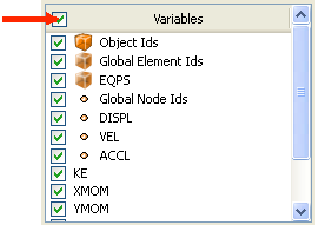
\includegraphics[scale=\bbscale]{images/Variables_can}
    \end{inlinefig}
  \item As before, click the checkbox in the header of the variable list to
    turn on the loading of all the variables and hit the \apply button.
  \item Press the~\yPlus button to orient the camera to the mesh.
  \item Press the play button~\vcrPlay in the toolbars and watch ParaView
    animate the mesh to crush the can with the falling brick.
  \end{enumerate}

  \begin{inlinefig}
    \includegraphics[width=.32\linewidth]{images/AnimateCan1}
    \includegraphics[width=.32\linewidth]{images/AnimateCan2}
    \includegraphics[width=.32\linewidth]{images/AnimateCan3}
  \end{inlinefig}
\end{exercise}

That is really all there is to dealing with data that is defined over time.
ParaView has an internal concept of time and automatically links in the
time defined by your data.  Become familiar with the toolbars that can be
used to control time.

\begin{inlinefig}
  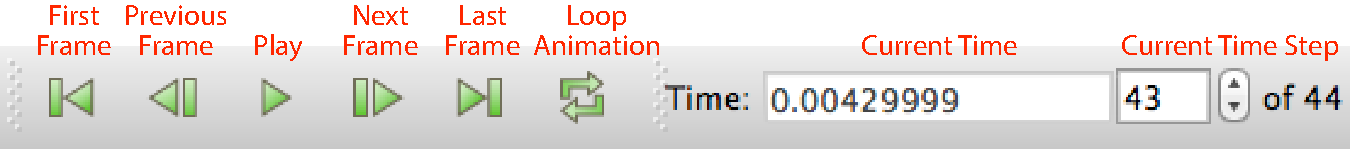
\includegraphics[width=\linewidth]{images/AnimationToolbar}
\end{inlinefig}

Saving an animation is equally as easy.  From the menu, select \gui{File}
\ra \gui{Save Animation}.  ParaView provides dialogs specifying how you
want to save the animation, and then automatically iterates and saves the
animation.

\begin{exercise}{Temporal Data Pitfall}
  \label{ex:TemporalDataPitfall}%
  The biggest pitfall users run into is that with mapping a set of colors
  whose range changes over time.  To demonstrate this, do the following.

  \begin{enumerate}
  \item If you are not continuing from
    Exercise~\ref{ex:LoadingTemporalData}, open the file \gui{can.ex2},
    load all variables, \apply.
  \item Go to the first time step~\vcrFirst.
  \item Turn on the \gui{EQPS} variable.
  \item Turn on the color legend~\icon{pqScalarBar32}.
  \item Play~\vcrPlay through the animation (or skip to the last time
    step~\vcrLast).
    \savecounter
  \end{enumerate}

  The coloring is not very useful.  To quickly fix the problem:

  \begin{enumerate}
    \restorecounter
  \item While at the last time step, click the Rescale to Data
    Range~\icon{pqResetRange24} button.
  \item Play~\vcrPlay the animation again.
  \end{enumerate}

  The colors are more useful now.
\end{exercise}

Although this behavior seems like a bug, it is not.  It is the consequence
of two unavoidable behaviors.  First, when you turn on the visibility of a
scalar field, the range of the field is set to the range of values in the
current time step.  Ideally, the range would be set to the max and min over
all time steps in the data.

However, this requires ParaView to load
in all of the data on the initial read, and that is prohibitively
slow for large data.  Second, when you animate over time, it is important
to hold the color range fixed even if the range in the data changes.
Changing the scale of the data as an animation plays causes a
misrepresentation of the data.  It is far better to let the scalars go out
of the original color maps range than to imply that they have not.  There
are several workarounds to this problem:

\begin{itemize}
\item Open the settings dialog box accessed in the menu from \gui{Edit} \ra
  \gui{Settings} (\gui{ParaView} \ra \gui{Preferences} on the Mac).  Under
  the \gui{General} tab, change the \gui{On File Open} setting to \gui{Goto
    last timestep}.  When this is selected, ParaView will automatically go
  to the last time step when loading any data set with time.  For many data
  (such as in can), the field ranges are more representative at the last
  time step than at the beginning.  Thus, as long as you color by a field
  before changing the time, the color range will be adequate.
\item If for whatever reason your animation gets stuck on a poor color
  range, simply go to a representative time step and
  hit~\icon{pqResetRange24}.
\item Alternatively, you can open the edit color scale dialog
  box~\icon{pqEditColor24} and specify a range for the data.  This is a
  good choice if you cannot find, or do not know, a ``representative'' time
  step or if you already know a good range to use.
\item If you are willing to wait, you can use the \gui{Rescale to Temporal
  Range} button on the edit color scale dialog box~\icon{pqEditColor24} and
  ParaView will compute this overall temporal range automatically.  Keep in
  mind that this option will require ParaView to load your entire data set
  over all time steps whenever you load a data set.  Although ParaView will
  not hold more than one time step in memory at a time, it will take a long
  time to pull all that memory off of disk for large data sets.
\end{itemize}


\section{Selection}

The goal of Visualization is often to find the important details within a
large body of information. ParaView's selection abstraction is an
important simplification of this process. Selection is the act of
identifying a subset of some dataset. There are a variety of ways that
this selection can be made, most of which are intuitive to end users,
and a variety of ways to display and process the specific qualities of
the subset once it is identified.

More specifically the subset identifies particular select points, cells, or
blocks within any single data set.  There are multiple ways of
specifying which elements to include in the selection including id
lists of multiple varieties, spatial locations, and scalar values and
scalar ranges.

In ParaView, selection can take place at any time, and the program
maintains a current selected set that is linked between all views.
That is, if you select something in one view, that selection is also
shown in all other views that display the same object.

The most direct means to create a selection is via the \gui{Find Data}
dialog. Launch this dialog from the \gui{Edit} menu.  From this dialog you
can enter characteristics of the data that you are seraching for.  For
example, you could look for points whose velocity magnitude is near
terminal velocity.  Or you could look for cells whose strain exceeds the
failure of the material.  The following exercise provides a quick example
of using the \gui{Find Data} dialog box.

\begin{exercise}{Data Element Selections vs. Spatial Selections}
  \label{ex:DataElementSelectionsVsSpatialSelections}%
  In this exercise we will find all cells with the large equivalent plastic
  strain (EQPS).

  \begin{enumerate}
  \item If you do not already have it loaded from the previous exercise,
    open the file \gui{can.ex2}, load all variables, \apply (see
    Exercise~\ref{ex:LoadingTemporalData}).
  \item Go to the last time step~\vcrLast.
  \item Open the find data dialog with \gui{Edit} \ra \gui{Find Data}.
  \item From the top combo box, choose to find \gui{Cell}s.
  \item In the next row of widgets, choose \gui{EQPS} from the first combo
    box, \gui{is~$>=$} from the second combo box, and enter \gui{1.5} in the
    final text box.
  \item Click the \gui{Run Selection Query} button.
  \end{enumerate}

  \begin{inlinefig}
    \includegraphics[width=\scw]{images/FindData}
  \end{inlinefig}

  Observe the spreadsheet below the \gui{Run Selection Query} button that
  gets populated with the results of your query.  Each row represents a
  cell and each column represents a field value or property (such as an
  identifier).

  You may also notice that several cells are highlighted in the 3D view of
  the main ParaView window.  These highlights represent the selection that
  your query created.  Close the \gui{Find Data} dialog and note that the
  selection remains.
\end{exercise}

One of the easiest ways of creating a selection is to pick elements right
inside the 3D view.  All of the 3D view selections are performed with a
\keyterm{rubber-band} selection.  That is, by clicking and dragging the
mouse in the 3D view, you will create a boxed region that will select
elements underneath it.  There are several types of rubber-band selection
that can be performed, and you initiate one by selecting one of the icons
in the selection controls toolbar or using one of the shortcut keys.  The
following 3D selections are possible.

\begin{description}
\item[\selectCellsOn Select Cells On (Surface)] Selects cells that are
  visible in the view.  (Shortcut: s)
\item[\selectPointsOn Select Points On (Surface)] Selects points that are
  visible in the view.
\item[\selectCellsThrough Select Cells Through (Frustum)] Selects all cells
  that exist under the rubber band.
\item[\selectPointsThrough Select Points Through (Frustum)] Selects all
  points that exist under the rubber band.
\item[\selectBlocks Select Blocks] Selects blocks in a
  multiblock data set.  (Shortcut: b)
\end{description}

The shortcuts s and b allow you to quickly select a cell or block,
respectively.  Use them by placing the mouse cursor somewhere in the
currently selected 3D view and hitting the appropriate key.  Then click on
the cell or block you want selected (or drag a rubber band over multiple
elements).

Feel free to experiment with the selections now.

\begin{inlinefig}
  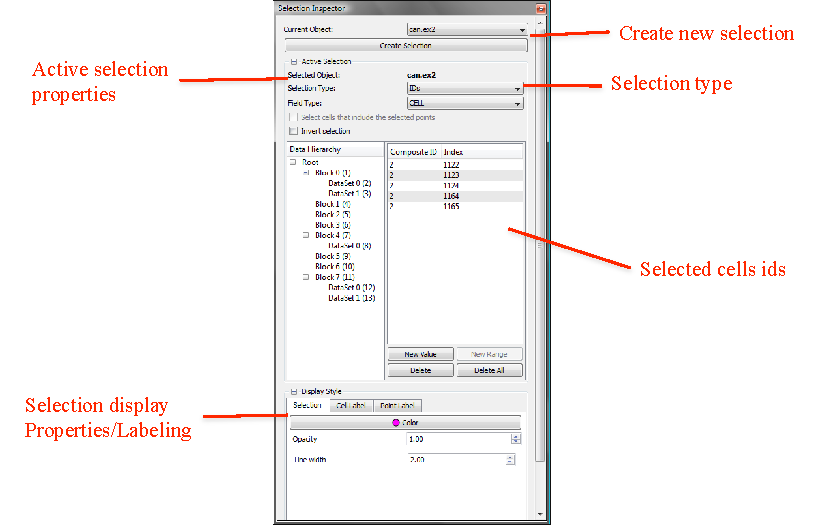
\includegraphics[scale=\bbscale]{images/SelectionInspector}
\end{inlinefig}

You can manage your selection with the \keyterm{selection inspector}.  You
can view the selection inspector through the menu \gui{View} \ra
\gui{Selection Inspector}.  The selection inspector allows you to view all
the points and cells in the selection as well as modify the selection.  You
can also use the selection inspector to add labels to the selection to make
it easier to identify which element is which.

Experiment with the selection inspector a bit.  Open the \gui{Selection
  Inspector}.  Then make selections using the rubber-band selection and see
the results in the \gui{Selection Inspector}.  Also experiment with
altering the selection by changing ids or inverting selections with the
\gui{Invert selection} checkbox.

You will notice that the select-on tools, \selectCellsOn/\selectPointsOn,
show a list of points/cells and the select blocks tool,~\selectBlocks,
shows a list of blocks, but the select-through tools,
\selectCellsThrough/\selectPointsThrough, show neither.  That is because it
is selecting a region in space.  If you click on the \gui{Show Frustum} and
rotate the 3D view to see the region of the selection.

It should be noted that there is a fundamental difference between
selections that specify a list of points or cells and a selection that
specifies a region in space.  The following exercise demonstrates the
difference.

\begin{exercise}{Data Element Selections vs. Spatial Selections}
  \label{ex:DataElementSelectionsVsSpatialSelections}%
  \begin{enumerate}
  \item If you do not already have it loaded from the previous exercise,
    open the file \gui{can.ex2}, load all variables, \apply (see
    Exercise~\ref{ex:LoadingTemporalData}).
  \item Make a selection using the \gui{Select Cells
    Through}~\selectCellsThrough tool.
  \item If it is not already visible, show the selection inspector
    with \gui{View} \ra \gui{Selection Inspector}.  You may need to dock
    the selection inspector elsewhere to see its widgets well.
  \item Click on the \gui{Show Frustum} checkbox in the \gui{Selection
    Inspector} and rotate the 3D view.

    \begin{inlinefig}
      \includegraphics[width=\scw]{images/SelectionFrustum}
    \end{inlinefig}

  \item Play~\vcrPlay the animation a bit.  Notice that the region remains
    fixed and the selection changes based on what cells move in or out of
    the region.
  \item Change the \gui{Selection Type} to \gui{IDs} in the \gui{Selection
    Inspector}.
  \item Play~\vcrPlay again.  Notice that the cells selected are fixed
    regardless of position.
  \end{enumerate}

  In summary, a spatial selection (created with one of the select through
  tools) will re-perform the selection at each time step as elements move
  in and out of the selected region.  Likewise, other queries such as field
  range queries will also reexecute as the data changes.  In contrast, in
  an ID selection, the points or cells selected are fixed and will be
  followed as they move through an animation.
\end{exercise}

The \keyterm{spreadsheet view} is an important tool to use in combination
with selections and quantitative drill down.  The spreadsheet view
allows you to read the actual values of scalar fields and the
selection mechanism will help you identify the values of interest.

\begin{exercise}{The Spreadsheet View and Selection}
  \label{ex:TheSpreadsheetViewAndSelection}%
  \begin{enumerate}
  \item If you do not already have it loaded from the previous exercise,
    open the file \gui{can.ex2}, load all variables, \apply (see
    Exercise~\ref{ex:LoadingTemporalData}).
  \item Split the view vertically~\splitViewV.
  \item In the new view, click the \gui{Spreadsheet View} button.
  \item Make \gui{can.ex2} visible (by clicking the appropriate \eyeballg)
    if not already visible.
    \savecounter
  \end{enumerate}

  As you can see, the spreadsheet view is fairly simple.  It shows the
  field data in tabular form for one field type (e.g. point or cell data)
  of one block of one data set.  This constraint is enforced to ensure that
  every row has the same column data.

  Note the widgets at the top of the spreadsheet view.  These let you
  quickly select the pipeline object, choose the type of field to show,
  choose the precision shown for floating point numbers, and hide
  everything but the selection.  As with any view, the spreadsheet view has
  its own \gui{Display} panels.

  \begin{inlinefig}
    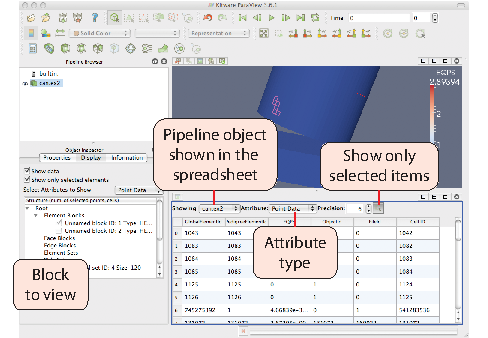
\includegraphics[scale=\bbscale]{images/SpreadsheetViewLabeled}
  \end{inlinefig}

  \begin{enumerate}
    \restorecounter
  \item In the \gui{Attribute} combo box, select \gui{Cell Data}.
  \item Scroll around the spreadsheet view and find some highlighted rows.
    (You may have to select a different block in the \gui{Display} panel.)
    \savecounter
  \end{enumerate}

  \begin{inlinefig}
    \includegraphics[width=\scw]{images/SpreadsheetViewExample}
  \end{inlinefig}

  Those highlighted rows are the ones that are part of the current
  selection.  This coordination of selection between views is an important
  mechanism to link views.  In this example, it can be difficult to identify
  the selected items in the spreadsheet view.  Often, you just want to see
  the data in the selection.

  \begin{enumerate}
    \restorecounter
  \item Click on the \gui{Show only selected elements}~\icon{pqSelect32}
    button at the top of the spreadsheet view.
    \savecounter
  \end{enumerate}

  We have now seen a selection made in the 3D view show up in the
  spreadsheet view.  The linking works in reverse as well.  We can make
  selections in the spreadsheet and they will be displayed in the 3D view.

  \begin{enumerate}
  \item Uncheck \gui{Show only selected elements}.
  \item Select a few rows in the spreadsheet view.
  \item Find the resulting selection in the 3D view.
  \end{enumerate}
\end{exercise}

The spreadsheet provides the most readable way to inspect field data.
However, sometimes it is helpful to place the field data directly in the 3D
view.  The next exercise describes how we can do that.

\begin{exercise}{Labeling Selections}
  \label{ex:LabelingSelections}%
  \begin{enumerate}
  \item If you do not already have it loaded from the previous exercise,
    open the file \gui{can.ex2}, load all variables, \apply (see
    Exercise~\ref{ex:LoadingTemporalData}).
  \item If you do not have a few cells selected from the previous exercise,
    select a few now. (For this exercise it is not a good idea to select a
    large amount of cells.)
  \item If it is not already visible, show the selection inspector
    with \gui{View} \ra \gui{Selection Inspector}.
  \item Click the \gui{Cell Label} tab in the \gui{Selection Inspector} (at
    the bottom).
  \item Check \gui{Visible}.
  \item Change the \gui{Label Mode} to \gui{EQPS}.
  \end{enumerate}

  \begin{inlinefig}
    \includegraphics[width=\scw]{images/SpreadsheetSelection}
  \end{inlinefig}

  ParaView places the values for the \gui{EQPS} field near the selected
  cell that contains that value.  It is also possible to change the look of
  the font with respect to type, size, and color through the selection
  inspector.
\end{exercise}

ParaView provides the ability to plot field data over time.  Because you
seldom want to plot everything over all time, these plots work against a
selection.

\begin{exercise}{Plot Over Time}
  \label{ex:PlotOverTime}
  \begin{enumerate}
  \item If you do not already have it loaded from the previous exercise,
    open the file \gui{can.ex2}, load all variables, \apply (see
    Exercise~\ref{ex:LoadingTemporalData}).
  \item If you do not have a few cells selected from the previous exercise,
    select a few now. (For this exercise it is not a good idea to select a
    large amount of cells.)
  \item With the selection still active, add the Plot Selection Over Time
    (\gui{Filters} \ra \gui{Data Analysis} \ra \gui{Plot Selection Over
    Time}~\icon{pqPlotCellOverTime24} or use the quick launch: ctrl+space
    Win/Linux, alt+space Mac). \index{plot~selection~over~time}
  \item \apply.
  \item Go to the \gui{Display} panel and select different blocks to plot
    (which correspond to each of the selected elements).
  \end{enumerate}

  \begin{inlinefig}
    \includegraphics[width=\scw]{images/PlotSelectionOverTime}
  \end{inlinefig}

  Note that the selection you had was automatically added as the selection
  to use in the \gui{Object Inspector}.  If you want to change the
  selection, simply make a new one and click \gui{Copy Active Selection} in
  the \gui{Object Inspector}.
\end{exercise}

You can also extract a selection in order to view the selected points or
cells separately or perform some independent processing on them.  This is
done through the \gui{Extract Selection}~\icon{pqExtractSelection24}
filter.

\begin{exercise}{Extracting a Selection}
  \label{ex:ExtractingASelection}%
  \begin{enumerate}
  \item If you do not already have it loaded from the previous exercise,
    open the file \gui{can.ex2}, load all variables, \apply (see
    Exercise~\ref{ex:LoadingTemporalData}).
  \item Turn off cell labels if they are still showing (check the
    \gui{Selection Inspector}).
  \item Make a sizable cell selection for example, with Select Cells
    Through~\selectCellsThrough.
  \item Create an \gui{Extract Selection}~\icon{pqExtractSelection24}
    filter (\gui{Filters} \ra \gui{Data Analysis} \ra \gui{Extract
      Selection} or use the quick launch: ctrl+space Win/Linux, alt+space
    Mac).  \index{extract selection}
  \item \apply.
  \end{enumerate}

  \begin{inlinefig}
    \includegraphics[width=\scw]{images/ExtractSelection}
  \end{inlinefig}

  The object in the view is replaced with the cells that you just
  selected. (Note that in this image I added a translucent surface and a
  second view with the original selection to show the extracted cells in
  relation to the full data.) You can perform computations on the extracted
  cells by simply adding filters to the extract selection pipeline object.
\end{exercise}

Now that we have finished the selection exercises, we will no longer be
using the \gui{Selection Inspector}.  You may close it now if you wish.


\section{Controlling Time}

% Originally this was in the Time section, but I had to move it due to a
% strange bug with the spreadsheet view and the temporal interpolator (bug
% 7701).  If that gets fixed, this section should probably go back up into
% the Time section (or at least before Selection).  Might also consider
% moving annotation before Selection so that you don't have to do that
% weird delete everything but can.

ParaView has many powerful options for controlling time and animation.  The
majority of these are accessed through the \keyterm{animation view}.  From
the menu, click on \gui{View} \ra \gui{Animation View}.

\begin{inlinefig}
  \includegraphics[width=\scw]{images/AnimationView}
\end{inlinefig}

For now we will examine the controls at the top of the animation view.  The
animation \keyterm{mode} parameter determines how ParaView will step
through time during playback.  There are three modes available.

\begin{description}
\item[Sequence] Given a start and end time, break the animation into a
  specified number of frames spaced equally apart.
\item[Real Time] ParaView will play back the animation such that it lasts
  the specified number of seconds.  The actual number of frames created
  depends on the update time between frames.
\item[Snap To TimeSteps] ParaView will play back exactly those time steps
  that are defined by your data.
\end{description}

Whenever you load a file that contains time, ParaView will automatically
change the animation mode to \gui{Snap To TimeSteps}.  Thus, by default you
can load in your data, hit play~\vcrPlay, and see each time step as defined
in your data.  This is by far the most common use case.

A counter use case can occur when a simulation writes data at variable time
intervals.  Perhaps you would like the animation to play back relative to
the simulation time rather than the time index.  No problem.  We can switch
to one of the other two animation modes.  Another use case is the desire to
change the playback rate.  Perhaps you would like to speed up or slow down
the animation.  The other two animation modes allow us to do that.

\begin{exercise}{Slowing Down an Animation with the Animation Mode}%
  \label{ex:SlowingDownAnAnimation}%
  We are going to start a fresh visualization, so if you have been
  following along with the exercises so far, now is a good time to reset
  ParaView.  The easiest way to do this is to press the~\disconnect button.

  \begin{enumerate}
  \item Open the file \gui{can.ex2}, load all variables, \apply (see
    Exercise~\ref{ex:LoadingTemporalData}).
  \item Press the~\yPlus button to orient the camera to the mesh.
  \item Press the play button~\vcrPlay in the toolbars.
    \savecounter
  \end{enumerate}

  During this animation, ParaView is visiting each time step in the
  original data file exactly once.  Note the speed at which the animation
  plays.

  \begin{enumerate}
    \restorecounter
  \item If you have not done so yet, make the animation view visible:
    \gui{View} \ra \gui{Animation View}.
  \item Change the animation mode to \gui{Real Time}.  By default the
    animation is set up with the time range specified by the data and a
    duration of 10 seconds.
  \item Play~\vcrPlay the animation again.
    \savecounter
  \end{enumerate}

  The result looks similar to the previous \gui{Snap To TimeSteps}
  animation, but the animation is now a linear scaling of the simulation
  time and will complete in 10 seconds.

  \begin{enumerate}
    \restorecounter
  \item Change the \gui{Duration} to 60 seconds.
  \item Play~\vcrPlay the animation again.
  \end{enumerate}

  The animation is clearly playing back more slowly.  Unless your computer
  is updating slowly, you will also notice that the animation appears
  jerkier than before.  This is because we have exceeded the temporal
  resolution of the data set.
\end{exercise}

Often showing the jerky time steps from the original data is the desired
behavior; it is showing you exactly what is present in the data.  However,
if you wanted to make an animation for a presentation, you may want a
smoother animation.

There is a filter in ParaView designed for this purpose.  It is called
the \keyterm{temporal interpolator}.  This filter will interpolate the
positional and field data in between the time steps defined in the original
data set.  This functionality is made possible by recent advances in the
ParaView and VTK pipeline structure.

\begin{exercise}{Temporal Interpolation}
  \label{ex:TemporalInterpolation}%
  This exercise is a continuation of Exercise~\ref{ex:VolumeRendering}.
  You will need to finish that exercise before beginning this one.

  \begin{enumerate}
  \item Make sure \gui{can.ex2} is highlighted in the pipeline browser.
  \item Select \gui{Filters} \ra \gui{Temporal} \ra \gui{Temporal
    Interpolator} or apply the \gui{Temporal Interpolator} filter using the
    quick launch (ctrl+space Win/Linux, alt+space Mac).
  \item \apply.
  \item Change back to \gui{Real Time} mode in the \gui{Animation
    Inspector} if necessary.
  \item Split the view~\splitViewH, show the \gui{TemporalInterpolator1} in
    one, show \gui{can.ex2} in the other, and link the cameras.
  \item Play~\vcrPlay the animation.
  \end{enumerate}

  You should notice that the output from the temporal interpolator animates
  much more smoothly than the original data.
\end{exercise}

It is worth noting that the temporal interpolator can (and often does)
introduce artifacts in the data.  It is because of this that ParaView will
never apply this type of interpolation automatically; you will have to
explicitly add the \gui{Temporal Interpolator}.  In general, mesh
deformations often interpolate well but moving fields through a static mesh
do not.  Also be aware that the \gui{Temporal Interpolator} only works if
the topology remains constant.  If you have an adaptive mesh that changes
from one time step to the next, the \gui{Temporal Interpolator} will give
errors.


\section{Text Annotation}

% This section should probably directly follow the material currently
% covered in the Controlling Time section.  If that material moves, so
% should this material.

When using ParaView as a communication tool it is often helpful to annotate
the images you create with text.  With ParaView it is very easy to create
text annotation wherever you want in a 3D view.  There is a special
\keyterm{text source} that simply places some text in the view.

\begin{exercise}{Adding Text Annotation}
  \label{ex:AddingTextAnnotation}%
  If you are continuing this exercise after finishing
  Exercise~\ref{ex:TemporalInterpolation}, feel free to simply continue.
  If you have had to restart ParaView since or your state does not match up
  well enough, it is also fine to start with a fresh state.

  \begin{enumerate}
  \item From the menu bar, select \gui{Sources} \ra \gui{Text}.
  \item In the text edit box of the object inspector, type a message.
  \item Hit the \apply button.
  \end{enumerate}

  \begin{inlinefig}
    \includegraphics[width=\scw]{images/TextSource}
  \end{inlinefig}

  The text you entered appears in the 3D view.  You can place this text
  wherever you want by simply dragging it with the mouse.  The
  \gui{Display} tab in the object inspector provides additional options for
  the size, font, and color of the text.  It also has additional controls
  for placing the text in the most common locations.

  \begin{inlinefig}
    \includegraphics[width=.66\scw]{images/TextPosition}
  \end{inlinefig}
\end{exercise}

Often times you will need to put the current time value into the text
annotation.  Typing the correct time value can be tedious an error prone
with the standard text source and impossible when making an animation.
Therefore, there is a special \keyterm{annotate time source} that will
insert the current animation time into the string.

\begin{exercise}{Adding Time Annotation}
  \label{ex:AddingTimeAnnotation}%
  \begin{enumerate}
  \item If you do not already have it loaded from a previous exercise, open
    the file \gui{can.ex2}, \apply.
  \item Add an \gui{Annotate Time} source (\gui{Sources} \ra \gui{Annotate
    Time} or use the quick launch: ctrl+space Win/Linux, alt+space Mac).
  \item Move the annotation around as necessary.
  \item Play~\vcrPlay and observe how the time annotation changes.
    \savecounter
  \end{enumerate}

  \begin{inlinefig}
    \includegraphics[width=\scw]{images/AnnotateTimeSource}
  \end{inlinefig}

  There are instances when the current animation time is not the same as
  the time step read from a data file.  Often it is important to know what
  the time stored in the data file is, and there is a special version of
  annotate time that acts as a filter.

  \begin{enumerate}
    \restorecounter
  \item Select \gui{can.ex2}.
  \item Use the quick launch (ctrl+space Win/Linux, alt+space Mac) to apply
    the \gui{Annotate Time Filter}. \index{annotate time filter}
  \item \apply.
  \item Move the annotation around as necessary.
  \item Check the animation mode in the \gui{Animation View}.  If it is set
    to \gui{Snap to TimeSteps}, change it to \gui{Real Time}.
  \item Play~\vcrPlay and observe how the time annotation changes.
  \end{enumerate}

  \begin{inlinefig}
    \includegraphics[width=\scw]{images/AnnotateTimeFilter}
  \end{inlinefig}
\end{exercise}


\section{Animations}

We have already seen how to animate a data set with time in it
(hit~\vcrPlay).  However, ParaView’s animation capabilities go far beyond
that.  With ParaView you can animate nearly any property of any pipeline
object.

\begin{exercise}{Animating Properties}
  \label{ex:AnimatingProperties}%
  We are going to start a fresh visualization, so if you have been
  following along with the exercises so far, now is a good time to reset
  ParaView.  The easiest way to do this is to press the~\disconnect button.

  \begin{enumerate}
  \item Create a sphere source (\gui{Sources} \ra \gui{Sphere}) and \apply it.
  \item Now make sure the animation view panel is visible (\gui{View} \ra
    \gui{Animation View} if it is not).
  \item Change the \gui{No. Frames} option to 50 (10 will go far too quickly).
  \item Find the property selection widgets at the bottom of the animation
    view and select \gui{Sphere1} in the first box and \gui{Start Theta} in
    the second box.
    \begin{inlinefig}
      \includegraphics[height=1.5\baselineskip]{images/AddStartThetaTrack}
    \end{inlinefig}
    Hit the \icon{pqPlus16} button.
  \end{enumerate}

  \begin{inlinefig}
    \includegraphics[width=.9\linewidth]{images/BuildAnimation1}
  \end{inlinefig}

  If you play~\vcrPlay the animation, you will see the sphere open up then
  eventually wrap around itself and disappear.

  \begin{inlinefig}
    \includegraphics[width=.2\linewidth]{images/AnimateSphere0}
    \includegraphics[width=.2\linewidth]{images/AnimateSphere1}
    \includegraphics[width=.2\linewidth]{images/AnimateSphere2}
    \includegraphics[width=.2\linewidth]{images/AnimateSphere3}
  \end{inlinefig}
\end{exercise}

What you have done is created a \keyterm{track} for the \gui{Start Theta}
property of the \gui{Sphere1} object.  A track is represented as horizontal
bars in the animation view.  They hold \keyterm{key frames} that specify
values for the property at a specific time instance.  The value for the
property is interpolated between the key frames.  When you created a track
two key frames were created automatically: a key frame at the start time
with the minimal value and a key frame at the end time with the maximal
value.  The property you set here defines the start range of the sphere.

You can modify a track by double clicking on it.  That will bring up a
dialog box that you can use to add, delete, and modify key frames.

\begin{inlinefig}
  \includegraphics[width=\scw]{images/AnimationKeyframesDialog}
\end{inlinefig}

Use this feature to create a new key frame in the animation.

\begin{exercise}{Modifying Animation Track Keyframes}
  \label{ex:ModifyingAnimationTrackKeyframes}%
  This exercise is a continuation of Exercise~\ref{ex:AnimatingProperties}.
  You will need to finish that exercise before beginning this one.

  \begin{enumerate}
  \item Double-click on the \gui{Sphere1 -- Start Theta} track.
  \item In the \gui{Animation Keyframes} dialog, click the \gui{New}
    button.  This will create a new key frame.
  \item Modify the first key frame value to be 360.
  \item Modify the second key frame time to be 0.5 and value to be 0.
  \item Click \gui{OK}.
  \end{enumerate}

  \begin{inlinefig}
    \includegraphics[width=.9\linewidth]{images/BuildAnimation2}
  \end{inlinefig}

  When you play the animation, the sphere will first get bigger and then get
  smaller again.
\end{exercise}

You are not limited to animating just one property.  You can animate any
number of properties you wish.  Now we will create an animation that
depends on modifying two properties.

\begin{exercise}{Multiple Animation Tracks}
  \label{ex:MultipleAnimationTracks}%
  This exercise is a continuation of Exercises \ref{ex:AnimatingProperties}
  and \ref{ex:ModifyingAnimationTrackKeyframes}.  You will need to finish
  those exercises before beginning this one.

  \begin{enumerate}
  \item Double-click on the \gui{Sphere1 -- Start Theta} track.
  \item In the \gui{Animation Keyframes} dialog, \gui{Delete} the first
    track (at time step 0).
  \item Click \gui{OK}.
  \item In the animation view, create a track for the \gui{Sphere1} object,
    \gui{End Theta} property.
  \item Double-click on the \gui{Sphere1 -- End Theta} track.
  \item Change the time for the second key frame to be 0.5.
  \end{enumerate}

  \begin{inlinefig}
    \includegraphics[width=.9\linewidth]{images/BuildAnimation3}
  \end{inlinefig}

  The animation will show the sphere creating and destroying itself, but this
  time the range front rotates in the same direction.  It makes for a very
  satisfying animation when you loop~\vcrLoop the animation.
\end{exercise}

In addition to animating properties for pipeline objects, you can animate
the camera.  ParaView provides methods for animating the camera along
curves that you specify.  The most common animation is to rotate the camera
around an object, always facing the object, and ParaView provides a means
to automatically generate such an animation.

\begin{exercise}{Camera Orbit Animations}
  \label{ex:CameraOrbitAnimations}%
  For this exercise, we will orbit the camera around whatever data you have
  loaded.  If you are continuing from the previous exercise, you are set
  up.  If not, simply load or create some data.  To see the effects, it is
  best to have asymmetry in the geometry you load.  \gui{can.ex2} is a good
  data set to load for this exercise.

  \begin{enumerate}
  \item Place the camera where you want the orbit to start.  The camera
    will move to the right around the viewpoint.
  \item Now make sure the animation view panel is visible (\gui{View} \ra
    \gui{Animation View} if it is not).
  \item In the property selection widgets, select \gui{Camera} in the first
    box and \gui{Orbit} in the second box.
    \begin{inlinefig}
      \includegraphics[height=1.5\baselineskip]{images/AddCameraOrbit}
    \end{inlinefig}
    Hit the \icon{pqPlus16} button.
    \savecounter
  \end{enumerate}

  \begin{inlinefig}
    \includegraphics[width=.66\scw]{images/CreateOrbitDialog}
  \end{inlinefig}

  Before the new track is created, you will be presented with a dialog box
  that specifies the parameters of the orbit.  The default values come from
  the current camera position, which is usually what you want.

  \begin{enumerate}
    \restorecounter
  \item Click \gui{OK}.
  \item Play~\vcrPlay.
  \end{enumerate}

  The camera will now animate around the object.
\end{exercise}


% Chapter Basic Usage
